\documentclass[aspectratio=169,unicode,dvipdfmx,14pt]{beamer}


\usepackage{url}
\usepackage{bm}
\usepackage{amsmath}
\usepackage{amssymb}
\usepackage{mathtools}
\usepackage{graphicx}
\usepackage[absolute,overlay]{textpos}
\usepackage{hyperref}
\usepackage{listings}
\usepackage{changepage}
\usepackage{lipsum}


\usefonttheme[onlymath]{serif}

\DeclareMathOperator*{\argmax}{argmax}

\DeclarePairedDelimiterX{\infdivx}[2]{(}{)}{%
  #1\;\delimsize\|\;#2%
}
\newcommand{\infdiv}{D_{\scriptsize \mbox{KL}}\infdivx}
\DeclarePairedDelimiter{\norm}{\lVert}{\rVert}

\hypersetup{
	setpagesize=false,
	bookmarksnumbered=true,%
	bookmarksopen=true,%
	colorlinks=true,%
	linkcolor=blue,
	citecolor=red,
}

\newcommand\FontMath{\fontsize{10}{12}\selectfont}
\renewcommand{\baselinestretch}{1.3}
\renewcommand{\familydefault}{\sfdefault}
\renewcommand{\kanjifamilydefault}{\gtdefault}
\usepackage[deluxe, expert]{otf}

\setbeamertemplate{navigation symbols}{}
\setbeamertemplate{footline}[frame number]
\setbeamerfont{footline}{size={\fontsize{15}{15}}}

\setbeamerfont{author}{size=\Large}
\setbeamerfont{institute}{size=\normalsize\itshape}
\setbeamerfont{title}{size=\huge}
\setbeamerfont{subtitle}{size=\LARGE\normalfont\slshape}


\title{ \\ベイズ推測(ベイズ推論)\\ Bayesian inference}
\author{\texorpdfstring{正田 備也\newline\href{mailto:masada@rikkyo.ac.jp}{masada@rikkyo.ac.jp}}{正田 備也}}
\date{}

\begin{document}

\begin{frame}
\titlepage
\end{frame}

\section{予測分布}

\begin{frame}\frametitle{Contents}
\Large \tableofcontents[currentsection]
\end{frame}

\begin{frame}{統計的推測 statistical inference}
\begin{itemize}
\item 観測データとして、$d$次元ユークリッド空間$\mathbb{R}^d$上の$n$個の点の集合$\bm{x}_1,\ldots,\bm{x}_N$が与えられているとする
\item 観測データをひとつの記号で$\mathcal{D}$と書くことにする
\begin{itemize}
\item つまり、$\mathcal{D}=\{ \bm{x}_1,\ldots,\bm{x}_N \}$
\end{itemize}
\item $\bm{x}_i$は、独立に同じ分布$q(\bm{x})$にしたがうと考えることにする
\begin{itemize}
\item つまり、$q(\mathcal{D}) = \prod_{i=1}^N q(\bm{x}_i)$
\end{itemize}
\item しかし、この分布$q(\bm{x})$を直接知る方法はない
\item そこで、$\mathcal{D}$から$q(\bm{x})$を推測することを、統計的推測ないし統計的学習という
\end{itemize}
\end{frame}

\begin{frame}{確率モデル probabilistic model}
\begin{itemize}
\item 真の分布を推測するとき、私たちは、あるパラメータ$\bm{\eta}$をもつ確率分布$p(\bm{x}|\bm{\eta})$を準備する
\begin{itemize}
\item $p(\bm{x}|\bm{\eta})$を確率モデルと呼ぶ
\end{itemize}
\item また、パラメータを決めること自体にも不確かさがあるとする場合、パラメータがしたがう事前分布$p(\bm{\eta})$も準備する
\begin{itemize}
\item 事前分布のパラメータ(ハイパーパラメータ)はまだ書かずにおく
\end{itemize}
\item このとき事後分布は以下のように書ける
\begin{align}
p(\bm{\eta} | \mathcal{D}) = \frac{1}{Z_N} p(\bm{\eta}) p(\mathcal{D}|\bm{\eta})
= \frac{1}{Z_N} p(\bm{\eta}) \prod_{i=1}^N p(\bm{x}_i | \bm{\eta})
\label{eq:posterior}
\end{align}
\item $Z_N$については次のスライドで
\end{itemize}
\end{frame}

\begin{frame}{周辺尤度}
\begin{itemize}
\item 式\eqref{eq:posterior}の事後分布の規格化定数$Z_N$を分配関数とも呼ぶ
\begin{itemize}
\item 分配関数partition functionは物理方面から来ている用語
\end{itemize}
\item $Z_N$は規格化定数なので$Z_N = \int p(\bm{\eta}) p(\mathcal{D}|\bm{\eta}) d\bm{\eta}$を満たす
\item つまり$Z_N = p(\mathcal{D})$
\item $p(\mathcal{D})$を、周辺尤度、もしくは、エビデンスevidenceと呼ぶ
\begin{itemize}
\item 論文ではmarginal likelihoodよりevidenceのほうをよく見かける
\end{itemize}
\item すなわち、事後分布は以下のようにも書ける
\begin{align}
p(\bm{\eta} | \mathcal{D}) = \frac{ p(\bm{\eta}) p(\mathcal{D}|\bm{\eta}) }{ p(\mathcal{D}) }
\end{align}
\end{itemize}
\end{frame}

\begin{frame}{観測データを生成する分布の推定(1/2)}
\begin{itemize}
\item 観測データ$\mathcal{D}$から、それを生成する分布$\hat{p}(\bm{x})$を推定する方法は、いろいろある
\item 観測データ$\mathcal{D}=\{\bm{x}_1,\ldots,\bm{x}_N\}$が与えられているとき、パラメータ$\bm{\eta}$の関数$\prod_{i=1}^N p(\bm{x}_i|\bm{\eta})$を尤度関数と呼ぶ
\item[1.] 尤度関数を最大にするパラメータ$\bm{\eta}_{\mbox{\scriptsize ML}}$を最尤推定量といい、$p(\bm{x} | \bm{\eta}_{\mbox{\scriptsize ML}})$を推測の結果$\hat{p}(\bm{x})$とする方法を、最尤推定という
\item[2.] 事後分布の最大値を与えるパラメータ$\bm{\eta}_{\mbox{\scriptsize MAP}}$を事後確率最大化推定量といい、$p(\bm{x} | \bm{\eta}_{\mbox{\scriptsize MAP}})$を推測の結果$\hat{p}(\bm{x})$とする方法を、事後確率最大化推定(もしくはMAP推定)という
\end{itemize}
\end{frame}

\begin{frame}{観測データを生成する分布の推定(2/2)}
\begin{itemize}
\item[3.] ベイズ的なモデリングの課題は事後分布を求めることだったが、
事後分布を使うと、以下で定義する予測分布$p(\bm{x}|\mathcal{D})$をもって推測の結果$\hat{p}(\bm{x})$とすることができる
\item 事後分布$p(\bm{\eta} | \mathcal{D})$によって確率モデル$p(\bm{x}|\bm{\eta})$を平均化したもの、
つまり、$p(\bm{\eta} | \mathcal{D})$に関する$p(\bm{x}|\bm{\eta})$の期待値を、予測分布と呼ぶ
\begin{align}
p(\bm{x}|\mathcal{D}) = \int p(\bm{x}|\bm{\eta}) p(\bm{\eta} | \mathcal{D}) d\bm{\eta}
\label{eq:predictive}
\end{align}
\end{itemize}
\end{frame}

\begin{frame}{ベイズ推測}
\begin{itemize}
\item ベイズ推測Bayesian inferenceとは、「真の分布は、おおよそ予測分布だろう」と推測することである
\begin{itemize}
\item[cf.] 渡辺澄夫『ベイズ統計の理論と方法』コロナ社、p.5
\end{itemize}
\item[] \ 
\item 以下、正規分布と多項分布の場合について、共役事前分布を使ったときに予測分布がどのような分布になるかを説明する
\end{itemize}
\end{frame}

\section{正規分布の場合}

\begin{frame}\frametitle{Contents}
\Large \tableofcontents[currentsection]
\end{frame}

\begin{frame}{単変量正規分布を使ったベイズ的モデリング}
\begin{itemize}
\item 観測データ$\mathcal{D}=\{x_1,\ldots,x_N\}$が独立に同じ正規分布$\mathcal{N}(\mu,\tau^{-1})$にしたがうと仮定
\item 平均$\mu$と精度$\tau$の事前分布として正規ガンマ分布$\mbox{NG}(\mu,\tau;\mu_0, \lambda_0, \alpha, \beta)$を使う
\item 正規ガンマ分布の確率密度関数は
\begin{align}
p(\mu, \tau ; \mu_0, \lambda_0, \alpha, \beta)
& = p(\mu | \tau ; \mu_0, \lambda_0, \alpha, \beta) p(\tau ; \alpha, \beta)
\notag \\ &
= \frac{\beta^\alpha\sqrt{\lambda_0}}{\Gamma(\alpha)\sqrt{2\pi}}
\tau^{\alpha-\frac{1}{2}}e^{-\beta\tau}e^{-\frac{\lambda_0\tau(\mu - \mu_0)^2}{2}}
\end{align}
\end{itemize}
\end{frame}

\begin{frame}{共役事前分布としての正規ガンマ分布 (1/2)}
\begin{itemize}
\item 正規ガンマ分布は共役事前分布
\item よって事後分布も正規ガンマ分布となる
\item 事後分布$p(\mu,\tau|\mathcal{D}; \mu_0, \lambda_0, \alpha, \beta)$は以下のように書ける
\begin{itemize}
\item 前回の講義資料を参照
\end{itemize}
\begin{align}
& p(\mu,\tau|\mathcal{D}; \mu_0, \lambda_0, \alpha, \beta) 
\notag \\ & \propto
\tau^{\alpha + \frac{N}{2} - \frac{1}{2}}
\exp \bigg[ - \tau \bigg( \beta + \frac{Ns}{2} + \frac{ \lambda_0 N (\bar{x} - \mu_0)^2 }{ 2( \lambda_0 + N ) }
\bigg) \bigg]
\notag \\ & \mbox{ \ }
\times \exp \bigg[ - \frac{\tau}{2} ( \lambda_0 + N ) \bigg( \mu - \frac{ \lambda_0 \mu_0 + N\bar{x} }{ \lambda_0 + N } \bigg)^2 \bigg]
\end{align}
\end{itemize}
\end{frame}


\begin{frame}{共役事前分布としての正規ガンマ分布 (2/2)}
\begin{itemize}
\item $N$を観測データの個数、$\bar{x} = \frac{\sum_{i=1}^N x_i}{N}$、$s=\frac{\sum_{i=1}^N (x_i - \bar{x})^2}{N}$とする。
\begin{itemize}
\item[cf.] \href{https://en.wikipedia.org/wiki/Normal-gamma_distribution}{https://en.wikipedia.org/wiki/Normal-gamma\_distribution} 
\end{itemize}
\end{itemize}
\begin{table}[t]
\caption{事前分布と事後分布とでのパラメータの値の対比}
\begin{center}
\begin{tabular}{|c|c|}
\hline
事前分布 & 事後分布 \\ \hline
$\mu_0$ & $\frac{ \lambda_0 \mu_0 + N\bar{x} }{ \lambda_0 + N }$ \\ 
$\lambda_0$ & $\lambda_0 + N$ \\
$\alpha$ & $\alpha + \frac{N}{2}$ \\
$\beta$ & $\beta + \frac{1}{2} \big( Ns + \frac{ \lambda_0 N (\bar{x} - \mu_0)^2 }{ \lambda_0 + N} \big)$ \\
\hline
\end{tabular}
\end{center}
\label{default}
\end{table}%
\end{frame}


\begin{frame}{予測分布}
\begin{itemize}
\item 上記の設定のもとでの予測分布$p(x | \mathcal{D})$は
$p(x|\mathcal{D}) = \int p(x|\mu,\tau)p(\mu,\tau|\mathcal{D}) d\mu d\tau$によって求められる
\item 事後分布は、$p(\mu,\tau|\mathcal{D})=p(\mu|\tau,\mathcal{D})p(\tau|\mathcal{D})$と、正規分布とガンマ分布の積で書ける(正規ガンマ分布だから)。よって
\begin{align}
p(x|\mathcal{D}) = \int p(x|\mu,\tau)p(\mu|\tau,\mathcal{D})p(\tau|\mathcal{D}) d\mu d\tau
\end{align}
\vspace{-.2in}
\begin{itemize}
\item $p(x|\mu,\tau) \propto \exp[ - \frac{\tau}{2} (x - \mu)^2 ]$
\item $p(\mu|\tau,\mathcal{D}) \propto \exp [ - \frac{\tau( \lambda_0 + N )}{2}  ( \mu - \frac{ \lambda_0 \mu_0 + N\bar{x} }{ \lambda_0 + N } )^2 ]$
\item $p(\tau|\mathcal{D}) \propto \tau^{\alpha + \frac{N}{2} - 1}
\exp [ - \tau ( \beta + \frac{Ns}{2} + \frac{ \lambda_0 N (\bar{x} - \mu_0)^2 }{ 2( \lambda_0 + N ) } ) ]$
\end{itemize}
\item この予測分布がどういう分布になるかを、以下で示す
\end{itemize}
\end{frame}

\begin{frame}{\textit{t}-分布 Student's \textit{t}-distribution}
\begin{itemize}
\item $x_1,\ldots,x_N$を平均$\mu$、標準偏差$\sigma$の正規分布に独立にしたがう確率変数とする
\item 標本平均を$\bar{x}=\frac{\sum_i x_i}{N}$、不偏分散を$s^2=\frac{\sum_i (x_i - \bar{x})^2}{N-1}$とする
\item このとき、$t = \frac{\bar{x} - \mu}{s / \sqrt{N}}$と定義される値は、自由度$\nu=N-1$の\textit{t}-分布にしたがう
\item \textit{t}-分布の確率密度関数は、以下のようになる
\begin{align}
p(t;\nu) = \frac{\Gamma((\nu+1)/2)}{\sqrt{\nu\pi}\Gamma(\nu/2)}(1 + t^2/\nu)^{-(\nu+1)/2}
\end{align}
\end{itemize}
\end{frame}

\begin{frame}{}
\begin{figure}[htbp]
\begin{center}
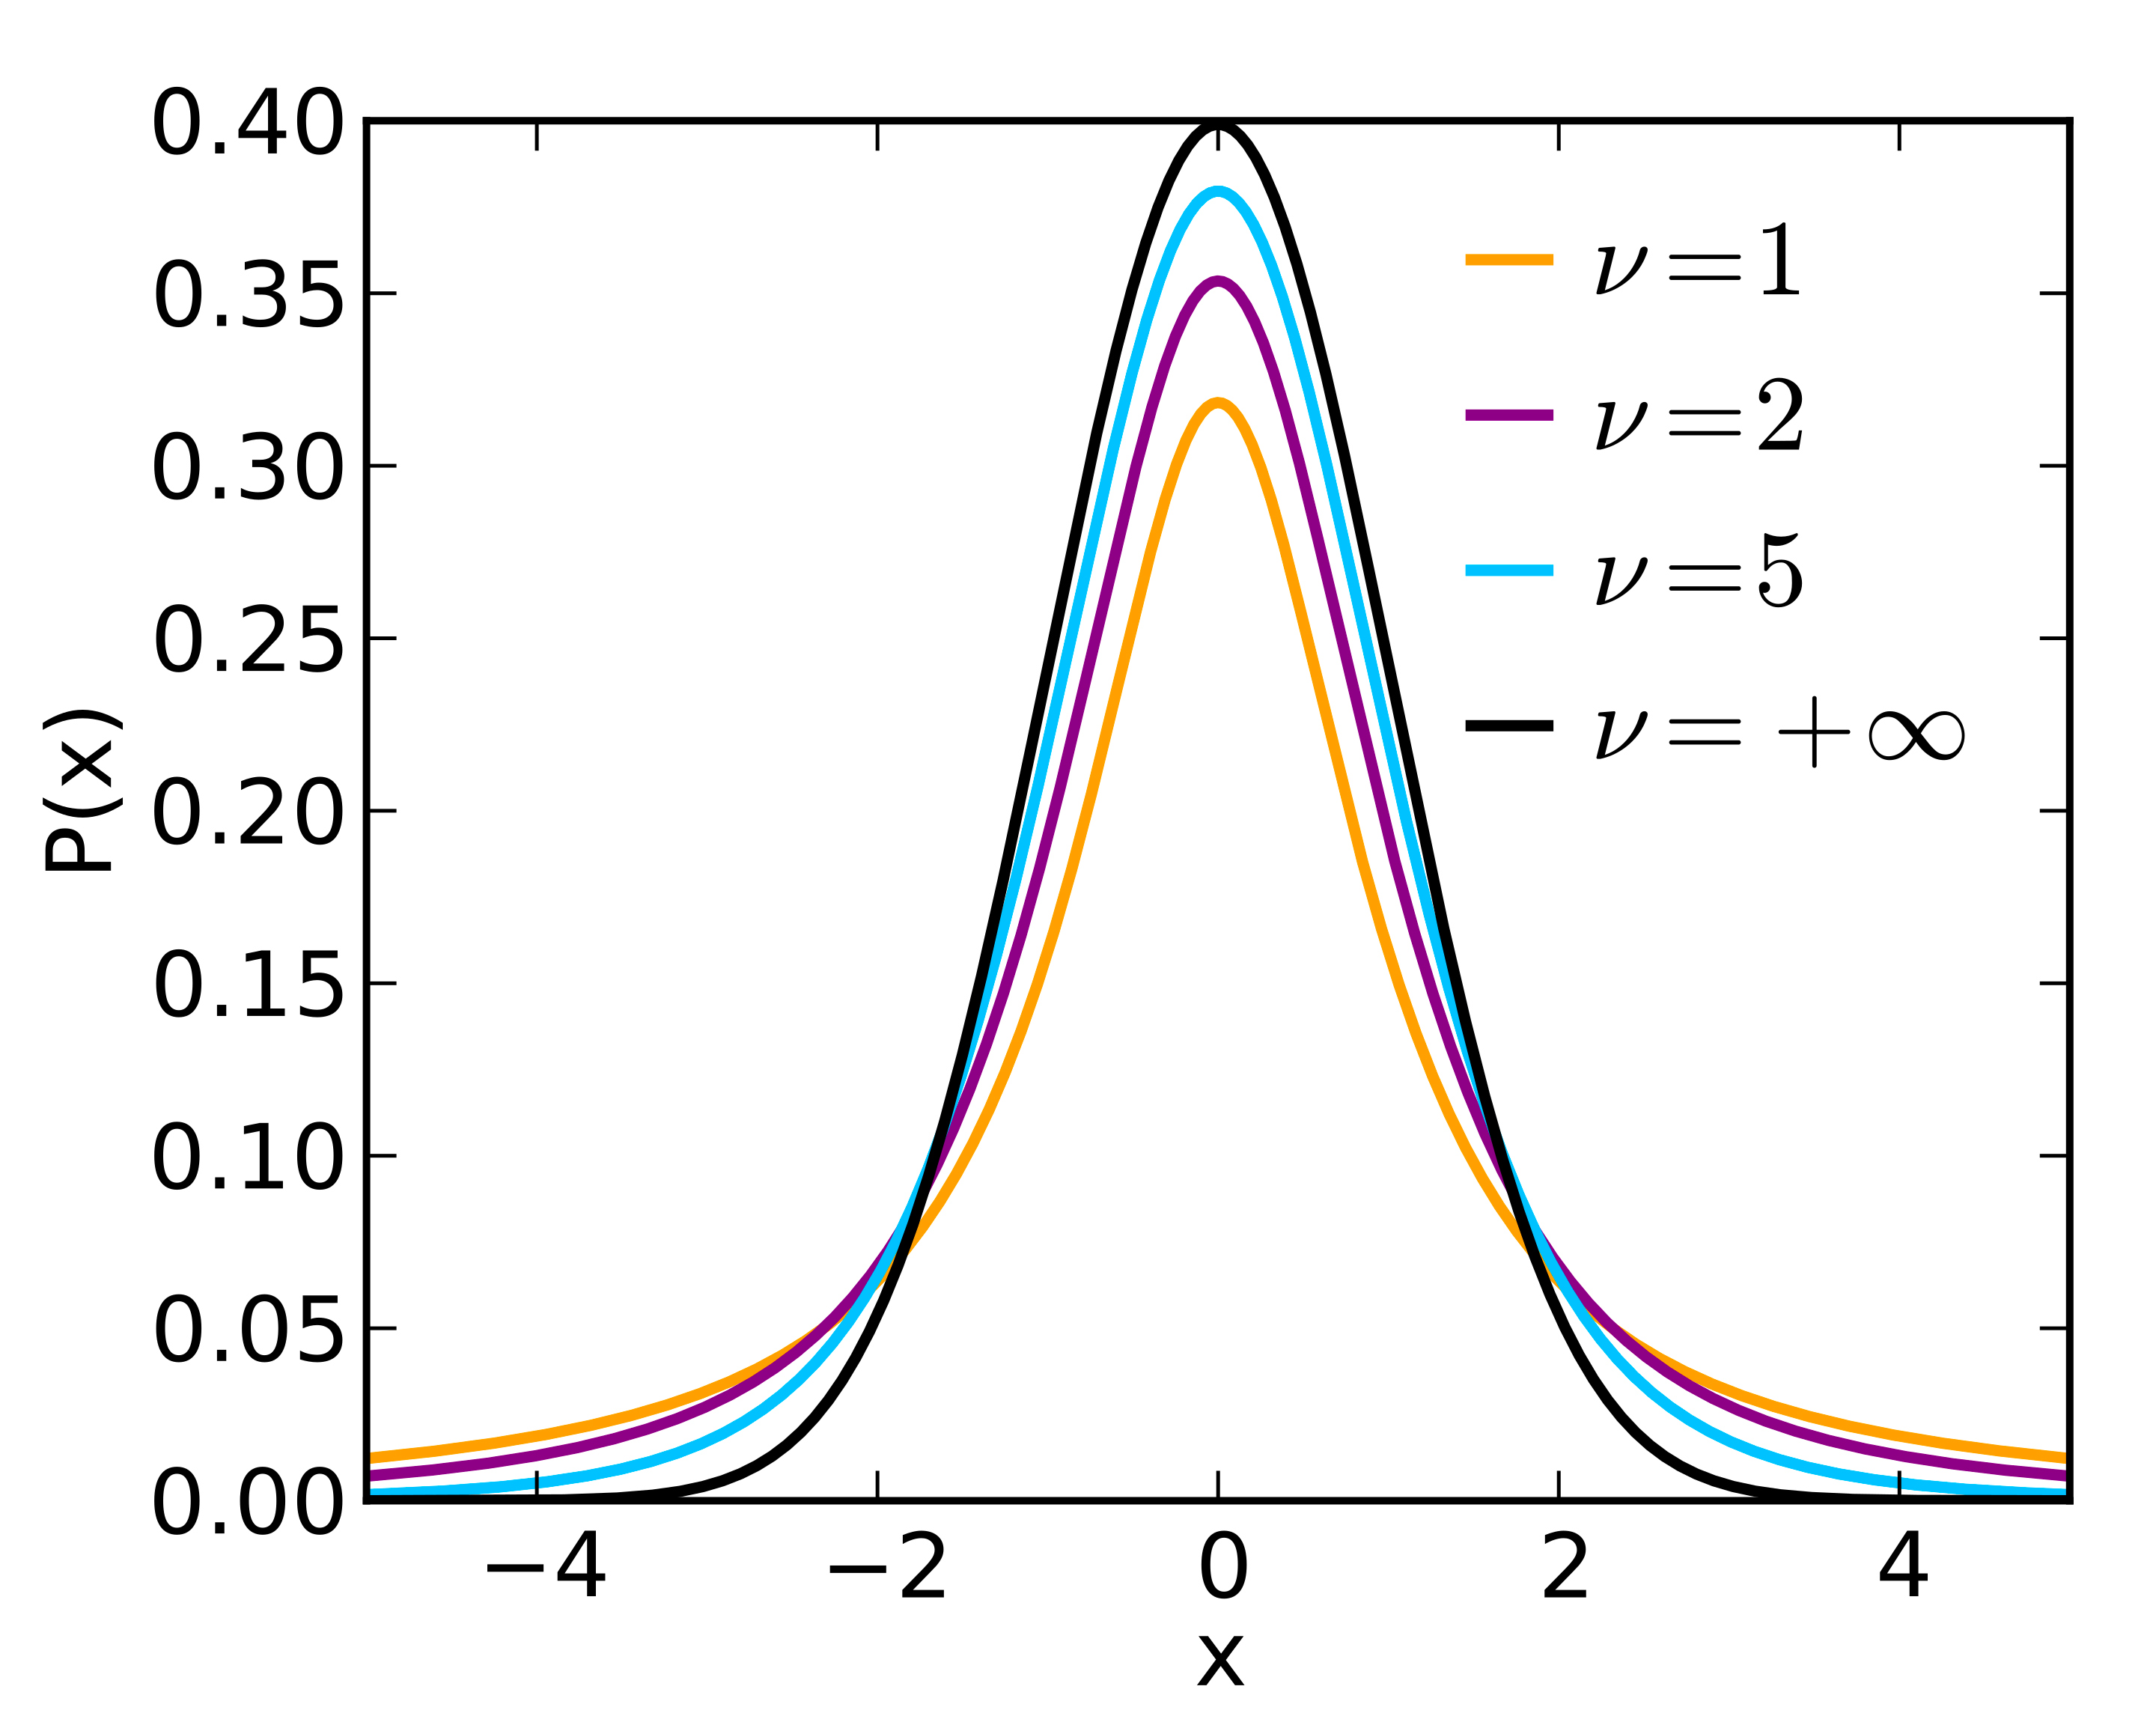
\includegraphics[scale=.09]{Student_t_pdf.jpg}
\caption{\href{https://en.wikipedia.org/wiki/Student's_t-distribution}{https://en.wikipedia.org/wiki/Student's\_t-distribution}}
\label{}
\end{center}
\end{figure}
\end{frame}


\begin{frame}{\textit{t} location-scale distribution}
\begin{itemize}
\item 平均が$\mu$、スケールが$\sigma^2$、自由度が$\nu$の\textit{t} location-scale distributionの確率密度関数は、以下のとおり
\begin{align}
p(x;\mu,\sigma^2) =\frac{\Gamma((\nu+1)/2)}{\sigma\sqrt{\nu\pi}\Gamma(\nu/2)} \bigg( 1 + \frac{(x - \mu)^2}{\nu\sigma^2} \bigg)^{ - (\nu+1) / 2 }
\end{align}
\item $\mu=0$、$\sigma=1$のとき、\textit{t}-分布に一致する
\begin{itemize}
\item 英語版Wikipedia「\href{https://en.wikipedia.org/wiki/Student's_t-distribution}{\textit{t}-分布}」の「\href{https://en.wikipedia.org/wiki/Student's_t-distribution\#Bayesian_inference}{4.2 Bayesian Inference}」を参照
\item MATLABの\href{https://www.mathworks.com/help/stats/prob.tlocationscaledistribution.html}{tLocationScaleDistributionの項}も参照
\end{itemize}
\item 以下では、予測分布がこの\textit{t} location-scale distributionになることを示す
\end{itemize}
\end{frame}


\begin{frame}
\FontMath
準備として、正規ガンマ分布$\mbox{NG}(\mu,\tau|\mu_0, \lambda_0, \alpha, \beta)$において
$\alpha=\beta=\frac{\nu}{2}$である場合、以下が成立することを確認しておく(証明はしない)。
(cf. \href{https://www.cs.ubc.ca/~murphyk/Teaching/CS340-Fall07/reading/NG.pdf}{CS340 (Machine learning) Fall 2007 @ UBC})
\begin{align}
t_\nu (\mu|\mu_0,\lambda_0^{-1}) = \int_0^\infty \mbox{NG}(\mu,\tau|\mu_0, \lambda_0, \frac{\nu}{2}, \frac{\nu}{2}) d\tau
= \int_0^\infty \mathcal{N}(\mu|\mu_0,(\lambda_0\tau)^{-1})\mbox{Ga}(\tau|\frac{\nu}{2},\frac{\nu}{2}) d\tau
\end{align}
ただし、$t_\nu (x|\mu,\sigma^2)$は、平均$\mu$、スケール$\sigma^2$、自由度$\nu$の\textit{t} location-scale distributionである。

$x \sim \mbox{Ga}(\alpha,\beta)$のとき、$cx \sim \mbox{Ga}(\alpha,\frac{\beta}{c})$となる。よって
\begin{align}
\int_0^\infty \mathcal{N}(\mu|\mu_0,(\lambda_0\tau)^{-1})\mbox{Ga}(\tau|\alpha,\beta) d\tau
& = \int_0^\infty \mathcal{N}(\mu|\mu_0,(\lambda_0\tau)^{-1})\mbox{Ga}(\tau|\alpha,\frac{\beta}{\alpha}\alpha) d\tau
\notag \\ & =
\int_0^\infty \mathcal{N}(\mu|\mu_0,(\lambda_0\tau)^{-1})\mbox{Ga}(\frac{\alpha}{\beta}\tau|\alpha,\alpha) d\tau
\notag \\ & =
\int_0^\infty \mathcal{N}(\mu|\mu_0,(\frac{\beta}{\alpha}\lambda_0\tau^\prime)^{-1})\mbox{Ga}(\tau^\prime|\alpha,\alpha) d\tau^\prime
\notag \\ & =
t_{2\alpha}(\mu|\mu_0,\frac{\beta}{\alpha\lambda_0})
\label{eq:t-dist}
\end{align}
\end{frame}

\begin{frame}
\FontMath
もうひとつの準備として、異なる二つの単変量正規分布の密度関数の積について、以下の結果を確認しておく。

この結果は、\href{https://www.johndcook.com/blog/2012/10/29/product-of-normal-pdfs/}{このブログ記事}において提示されているものだが、\href{https://www.ics.uci.edu/~welling/teaching/KernelsICS273B/MatrixCookBook.pdf}{The Matrix Cookbook}の7.2.6.で提示されている結果の特殊例でもある。

\ \\
平均が$m$で標準偏差が$s$の単変量正規分布の密度関数を$f(x;m,s)$と書くことにすると
\begin{align}
f(x;\mu_1,\sigma_1)f(x;\mu_2,\sigma_2) 
= f\Big(\mu_1;\mu_2,\sqrt{\sigma_1^2+\sigma_2^2}\Big) f(x;\mu,\sigma)
\end{align}
ただし、
\begin{align}
\mu & =\frac{\sigma_1^{-2}\mu_1 + \sigma_2^{-2}\mu_2}{\sigma_1^{-2} + \sigma_2^{-2}} \\
\sigma^2 &= \frac{\sigma_1^2\sigma_2^2}{\sigma_1^2 + \sigma_2^2}
\end{align}
\end{frame}


\begin{frame}
\FontMath
$p(\mu|\tau,\mathcal{D}) \propto \exp [ - \frac{\tau( \lambda_0 + N )}{2}  ( \mu - \frac{ \lambda_0 \mu_0 + N\bar{x} }{ \lambda_0 + N } )^2 ]$において$\mu_N = \frac{ \lambda_0 \mu_0 + N\bar{x} }{ \lambda_0 + N }, \tau_N = \tau(\lambda_0 + N)$とおく。

前のスライドの結果を使うべく、$\mu_1 = x, \sigma_1 = \tau^{-1/2}, \mu_2 = \mu_N, \sigma_2 = \tau_N^{-1/2}$とおくと
\begin{align}
& p(x|\mu,\tau) p(\mu|\tau,\mathcal{D})
\propto
\exp\bigg[ - \frac{ \tau\tau_N }{2(\tau + \tau_N)} (x - \mu_N)^2 \bigg]
\exp\bigg[ - \frac{ \tau + \tau_N }{2} \Big(\mu - \frac{ \tau_N x + \tau \mu_N }{ \tau + \tau_N }\Big)^2 \bigg]
\notag \\ & =
\exp\bigg[ - \frac{ \tau( \lambda_0 + N ) }{2(\lambda_0 + N + 1)} (x - \mu_N)^2 \bigg]
\exp\bigg[ - \frac{ \tau( \lambda_0 + N + 1 ) }{2} \Big(\mu - \frac{ ( \lambda_0 + N ) x + \mu_N }{ \lambda_0 + N + 1 }\Big)^2 \bigg]
\end{align}
よって、$\alpha_N=\alpha+\frac{N}{2}, \beta_N = \beta + \frac{Ns}{2} + \frac{ \lambda_0 N (\bar{x} - \mu_0)^2 }{ 2( \lambda_0 + N ) }$、さらに$\lambda_N = \lambda_0 + N$とおくと、
\begin{align}
& p(x|\mu,\tau) p(\mu|\tau,\mathcal{D})p(\tau|\mathcal{D})
\propto
\exp\bigg[ - \frac{ \tau( \lambda_0 + N ) }{2(\lambda_0 + N + 1)} (x - \mu_N)^2 \bigg]
\notag \\ & \mbox{ \ } \times
\exp\bigg[ - \frac{ \tau( \lambda_0 + N + 1 ) }{2} \Big(\mu - \frac{ ( \lambda_0 + N ) x + \mu_N }{ \lambda_0 + N + 1 }\Big)^2 \bigg] \times
\tau^{\alpha_N - 1} e^{ - \tau \beta_N }
\notag \\ & \mbox{ \ } = \tau^{\alpha_N - 1} e^{ - \tau \beta_N }
\exp\bigg[ - \frac{ \tau \lambda_N }{2(\lambda_N + 1)} (x - \mu_N)^2 \bigg]
\times \exp\bigg[ - \frac{ \tau( \lambda_N + 1 ) }{2} \Big(\mu - \frac{ \lambda_N x + \mu_N }{ \lambda_N + 1 }\Big)^2 \bigg]
\end{align}
\end{frame}

\begin{frame}
\FontMath
$\mu$を積分消去すると
\begin{align}
p(x, \tau|\mathcal{D})
= \int_{-\infty}^\infty p(x|\mu,\tau) p(\mu|\tau,\mathcal{D})p(\tau|\mathcal{D}) d\mu
\propto
\tau^{\alpha_N - \frac{1}{2}}
e^{ - \tau \beta_N } \exp\bigg[ - \frac{ \tau \lambda_N }{2(\lambda_N + 1)} (x - \mu_N)^2 \bigg]
\end{align}
この式は$p(x, \tau|\mathcal{D})$が正規ガンマ分布の密度関数であることを示している。

そこで、$\tau$を積分消去するために式\eqref{eq:t-dist}の結果を使うと、
\begin{align}
p(x|\mathcal{D}) = \int p(x, \tau|\mathcal{D}) d\tau
= t_{2\alpha_N} ( x | \mu_N, \frac{\beta_N(\lambda_N + 1)}{\alpha_N\lambda_N} ) 
\end{align}
したがって、予測分布は、平均$\mu_N$、スケール$\frac{\beta_N(\lambda_N + 1)}{\alpha_N\lambda_N}$、自由度$2\alpha_N$の\textit{t} location-scale distributionである。
\end{frame}

\section{多項分布の場合}

\begin{frame}\frametitle{Contents}
\Large \tableofcontents[currentsection]
\end{frame}

\begin{frame}{多項分布を使ったベイズ的モデリング}
\begin{itemize}
\item 観測データ$\bm{x}=\{x_1,\ldots,x_n\}$が独立に同じカテゴリカル分布$\mbox{Cat}(\bm{\phi})$にしたがうと仮定
\begin{itemize}
\item 例えば、$x_{62} = \mbox{``apple''}$は、62番目に出現した単語が``apple''だ、という意味
\end{itemize}
\item $\bm{\phi}$の事前分布としてディリクレ分布$\mbox{Dir}(\bm{\beta})$を使う
\item ディリクレ分布の確率密度関数は
\begin{align}
p(\bm{\phi}; \bm{\beta}) = \frac{\Gamma(\sum_{w=1}^W \beta_w)}{\prod_{w=1}^W \Gamma(\beta_w)}
\prod_{w=1}^W \phi_W^{\beta_w - 1}
\end{align}
\end{itemize}
\end{frame}

\begin{frame}{共役事前分布としてのディリクレ分布}
\begin{itemize}
\item 正規ガンマ分布は共役事前分布
\item よって事後分布も正規ガンマ分布となる
\item 事後分布$p(\bm{\phi}|\bm{x}; \bm{\beta})$は以下のように書ける
\begin{align}
p(\bm{\phi}|\bm{x}; \bm{\beta}) = 
\frac{\Gamma(\sum_{w=1}^W (c_w + \beta_w))}{\prod_{w=1}^W \Gamma(c_w + \beta_w)}
\prod_{w=1}^W \phi_W^{c_w + \beta_w - 1}
\end{align}
\end{itemize}
\end{frame}

\begin{frame}{予測分布}
\begin{itemize}
\item 多項分布の場合、予測分布についても、多数の単語出現からなる観測データの予測分布を考えることが多い
\item その予測分布を求めたい単語列(つまり文書)を$\bm{x}_0$とする
\item $\bm{x}_0 = \{x_{0,1}, \ldots, x_{0,n_0}\}$とする。
\item 上記の設定のもとでの予測分布$p(\bm{x}_0 | \bm{x};\bm{\beta})$は
$p(\bm{x}_0|\bm{x};\bm{\beta}) = \int p(\bm{x}_0|\bm{\phi})p(\bm{\phi}|\bm{x};\bm{\beta}) d\bm{\phi}$によって求められる
\item この予測分布がどういう分布になるかを、以下で示す
\end{itemize}
\end{frame}

\begin{frame}
\FontMath
\begin{align}
& p(\bm{x}_0|\bm{x};\bm{\beta}) = \int p(\bm{x}_0|\bm{\phi})p(\bm{\phi}|\bm{x};\bm{\beta}) d\bm{\phi}
\notag \\ & =
\int \bigg(
\frac{n_0!}{\prod_{w=1}^W c_{0,w}!} \prod_{w=1}^W \phi_w^{c_{0,w}} \times
\frac{\Gamma(\sum_{w=1}^W (c_w + \beta_w))}{\prod_{w=1}^W \Gamma(c_w + \beta_w)}
\prod_{w=1}^W \phi_W^{c_w + \beta_w - 1} \bigg) d\bm{\phi}
\notag \\ & =
\frac{n_0!}{\prod_{w=1}^W c_{0,w}!}
\frac{\Gamma(\sum_{w=1}^W (c_w + \beta_w))}{\prod_{w=1}^W \Gamma(c_w + \beta_w)}
\int \prod_{w=1}^W \phi_W^{c_w + c_{0,w} + \beta_w - 1} d\bm{\phi}
\notag \\ & =
\frac{n_0!}{\prod_{w=1}^W c_{0,w}!}
\frac{\Gamma(\sum_{w=1}^W (c_w + \beta_w))}{\prod_{w=1}^W \Gamma(c_w + \beta_w)}
\frac{\prod_{w=1}^W \Gamma(c_w+c_{0,w}+\beta_w)}
{\Gamma( \sum_{w=1}^W (c_w + c_{0,w} + \beta_w) )}
\notag \\ & =
\frac{n_0! \Gamma(\sum_{w=1}^W (c_w + \beta_w))}{\Gamma( \sum_{w=1}^W (c_w + c_{0,w} + \beta_w) )}
\prod_{w=1}^W
\frac{\Gamma(c_w+c_{0,w}+\beta_w)}{c_{0,w}!\Gamma(c_w + \beta_w)}
\notag \\ & =
\frac{n_0 (n_0-1) \cdots 2 \cdot 1}{( n+n_0-1+\beta_\Sigma)( n+n_0-2+\beta_\Sigma) \cdots (n+1+\beta_\Sigma)(n + \beta_\Sigma)}
\notag \\ & \mbox{ \ \ } \times
\prod_{w=1}^W
\frac{(c_w+c_{0,w}-1+\beta_w)(c_w+c_{0,w}-2+\beta_w)\cdots(c_w+1+\beta_w)(c_w+\beta_w) }
{c_{0,w} (c_{0,w} - 1) \cdots 2 \cdot 1}
\end{align}
\end{frame}

\begin{frame}{ディリクレ多項分布(Polya分布)}
\begin{itemize}
\item パラメータは
$\bm{\alpha} = (\alpha_1, \ldots, \alpha_K)$ s.t. $\alpha_k > 0$ for $1 \leq k \leq K$
\item 確率密度関数は
\begin{align}
p(\bm{x} | \bm{\alpha}) = \frac{\Gamma(\sum_k \alpha_k)}{\prod_k \Gamma(\alpha_k)}
\frac{\prod_k \Gamma(\alpha_k + n_k)}{\Gamma(\sum_k \alpha_k + n_k)}
\end{align}
\vspace{-.1in}
\begin{itemize}
\item $n_k$は$\bm{x}$において第$k$番目のアイテムが出現する回数
\end{itemize}
\item 導出
\begin{align}
p(\bm{x} | \bm{\alpha}) = \int p(\bm{x}|\bm{\theta}) p(\bm{\theta} | \bm{\alpha}) d\bm{\theta}
\end{align}
\vspace{-.2in}
\begin{itemize}
\item $p(\bm{x}|\bm{\theta})$はパラメータが$\bm{\theta}$の多項分布の確率質量関数
\item $p(\bm{\theta} | \bm{\alpha})$はパラメータが$\bm{\alpha}$のディリクレ分布の確率密度関数
\end{itemize}
\end{itemize}
\end{frame}

\section{まとめ}

\begin{frame}\frametitle{Contents}
\Large \tableofcontents[currentsection]
\end{frame}

\begin{frame}{まとめ:予測分布とは何だったか}
\begin{itemize}
\item 事前分布$p(\bm{\eta})$と尤度$p(\mathcal{D}|\bm{\eta})$から、
事後分布$p(\bm{\eta} | \mathcal{D})$を求める
\begin{align}
p(\bm{\eta} | \mathcal{D}) = \frac{1}{Z_N} p(\bm{\eta}) p(\mathcal{D}|\bm{\eta})
= \frac{1}{Z_N} p(\bm{\eta}) \prod_{i=1}^N p(\bm{x}_i | \bm{\eta})
\end{align}
\vspace{-.2in}
\begin{itemize}
\item 事後分布$p(\bm{\eta} | \mathcal{D})$は、モデルパラメータが取りうるあらゆる値に重み付けをしている、
と見なせる
\end{itemize}
\item 下記の予測分布$p(\bm{x}|\mathcal{D})$を使うと、
事後分布$p(\bm{\eta} | \mathcal{D})$によるパラメータへの重み付けを反映するかたちで、
未知データ$\bm{x}$の確率を計算できる
\begin{align}
p(\bm{x}|\mathcal{D}) = \int p(\bm{x}|\bm{\eta}) p(\bm{\eta} | \mathcal{D}) d\bm{\eta}
\end{align}
\end{itemize}
\end{frame}

\begin{frame}{予測分布の別の見方}
\begin{itemize}
\item 予測分布を求めることは、観測データがしたがう新しい分布をベイズ的な枠組みを使って作り出すこと、とも言える
\item[1.] 正規分布と正規ガンマ分布から、\textit{t} location-scale 分布
\item[2.] 多項分布とディリクレ分布から、ディリクレ多項分布 
\begin{itemize}
\item ただし、今回の2つの例のように、予測分布の確率密度関数を式の計算で求めることができてしまうケースは、多くない
\end{itemize}
\end{itemize}
\end{frame}


\end{document}